\documentclass{article}
\usepackage{graphicx,xy,amsmath,amssymb,amsthm,physics,mathtools,tcolorbox,hyperref}
\usepackage{xepersian}
\settextfont{XB Niloofar}
\renewcommand{\contentsname}{هفته های تدریس}
\title{	
	پیش گزارش سوم درس آزمایشگاه اپتیک - دکتر مهدوی
	\\
	\small
	موضوع آزمايش: مطالعه تيغه هاي بازدارنده ربع موج، نيم موج، تمام موج و بررسی قانون مالوس
}
\author{
حسین محمدی 
\\
۹۶۱۰۱۰۳۵
}
\begin{document}
\maketitle
\section{هدف آزمایش}
در این آزمایش باز هم با وسایل پایه ای آزمایشگاه اپتیک آشنا می شویم و این وسیله های قطبشگرها هستند. ابتدا با تیغه های ربع موج، نیم موج و تمام موج و شیوه ی عملکرد آن ها(تغییر قطبش در اثر عبور نور از آن ها)آشنا می شویم و سپس با این شناختی که از این تیغه ها به دست می آوریم؛ سعی می کنیم با داده های آزمایشگاهی، چند تیغه ی مجهول را شناسایی کنیم. در نهایت هم قانون مالوس را بررسی می کنیم که رابطه بین شدت نور ورودی به قطبشگر و نور خروجی از آن است.

\noindent  \\
به طور دقیق تر
\begin{itemize}
	\item  اثر تیغه ربع موج بر نور قطبیده خطی
	\item تعیین نوع چهار تیغه مجهول
	\item ترکیب دو تیغه ربع موج
	\item بررسی قانون مالوس
\end{itemize}
\section{معرفی مختصر تیغه های ربع موج، نیم موج و تمام موج}
این تیغه ها تماما بلورهایی دوشکستی هستند و می دانیم که در «بلورهای دوشکستی» ضریب شکست نور در دو راستای معین، متفاوت است(که معمولا در همان راستاها برش می خورند و به شکل متوازی السطوح هستند) و همین باعث می شود که نوری که  از این تیغه عبور می کند، هنگام خروج از آن دو راستای معین شده دچار اختلاف راه (یا اختلاف فاز) شده و که با این اختلاف فاز، دسته بندی تیغه ها ر انجام می دهیم.

\noindent
\begin{itemize}
	\item
	اگر اختلاف فاز ایجاد شده
	$\frac{\pi}{2}$
	باشد تیغه را ربع موج می نامیم.
	\item اگر این اختلاف فاز برابر با 
	$\pi$
	باشد این تیغه را نیم موج می نامیم.
	\item
	اگر اختلاف فاز مذکور برابر با 
	$2\pi$
	باشد، تیغه تمام موج نامیده می شود.
\end{itemize}
\section{چگونگی تبدیل نور قطبیده خطی به دایروی}
فرض کنید که نور قطبیده ی خطی را داریم که به تیغه ی ربع موج برخورد کند، در این صورت معادله ی میدان آن به شکل 
$\vec{P} = \vec{P_0}\cos (\omega t)$ 
است. اگر بردار 
$\vec{P_0}$
با محور مثبت 
$x$
زاویه ی 
$\alpha$ بسازد، در این صورت تجزیه این میدان روی محورهای به شکل زیر است.
\[
\vec{P} = (P_0 \cos(\alpha)\cos (\omega t) ,P_0 \sin(\alpha)\cos (\omega t))
\]
و 
$|\vec{P_0}| = P_0$
اما پس از عبور از تیغه ربع موج، در یکی از جهت ها دچار اختلاف فاز 
$\frac{\pi}{2}$
می شود و داریم:
\[
x^{'} = P_0 \cos(\alpha)\cos (\omega t)
\]
\[
y^{'} = P_0 \sin(\alpha)\cos (\omega t - \frac{\pi}{2}) = - P_0 \sin(\alpha)\sin (\omega t)
\]
که معادله ی پارامتری یک دایره می شود و این یعنی که قطبش به شکل دایروی است.
\begin{figure}[h]
	\centering
	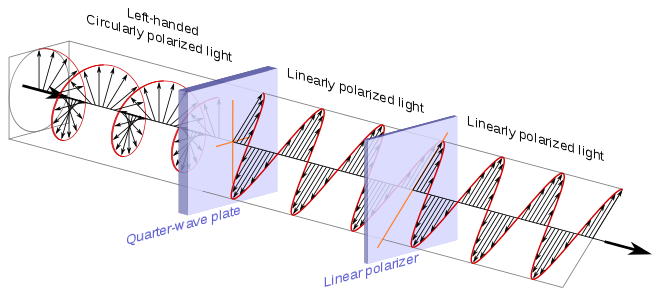
\includegraphics[width=\linewidth]{1.png}
	\caption{قطبش خطی و عبور از تیغه نیم موج و قطبش دایروی}
	\label{Fig1}
\end{figure}
\section{طرز کار یک تیغه قطبشگر خطی}
چطور است که قطبشگر، نور با یک قطبش خاص را عبور می دهد و اجازه عبور به سایر قطبش ها را نمی دهد؟

\noindent\\
از همین بلورهای دو شکستی که در بالا معرفی کرده ایم می توانیم برای ساخت یک قطبشگر استفاده کرد؛ به این صورت که دستگاهی تعبیه کنیم یکی موج خروجی از یکی از راستاهای را اجازه خروج ندهد یعنی 
\lr{Block}
 شود و نور دیگر را اجازه خروج دهد.
 













\end{document}